\documentclass{article}
\usepackage[portuguese]{babel}
\usepackage[latin1]{inputenc}
\usepackage{cite}
\usepackage{graphicx}
\usepackage[english,num,USenglish]{isodate}

\begin{document}
	\begin{titlepage}
	\centering
	\fontsize{12}{18}
	\fontfamily{ptm}
	\selectfont
		UNIVERSIDADE FEDERAL DO RIO GRANDE DO NORTE\\
		DEPARTAMENTO DE COMPUTA��O E AUTOMA��O\\
		INTELIG�NCIA ARTIFICIAL\\
		PROFESSOR MARCELO AUGUSTO COSTA FERNANDES\\[20 mm]
		ANDRESSA ST�FANY S. DE OLIVEIRA - 20160154101\\
		VITOR RAMOS GOMES DA SILVA - 20160154415\\[50 mm]
	\fontsize{18}{18}	
	\selectfont
		RELAT�RIO DO PROJETO
		3� UNIDADE
	\vfill
	\fontsize{12}{18}
	\selectfont
	\printdate{2016-12-04}
	\end{titlepage}
	
	\newpage
	\tableofcontents
	\newpage
	\section{Resumo}
	\paragraph{} \hspace{8pt}
		A problem�tica � a cerca de um rob�, que a priori n�o tem conhecimento dos obst�culos presentes no cen�rio. Com a utiliza��o de regras de produ��o, o rob� � capaz de se desviar dos obst�culos, para isso, fez-se uso do sensor Sonar, o qual informa as dist�ncias livres em sua frente, tr�s, esquerda e direita. Esses dados s�o utilizados como entradas nos sistemas especialistas e como sa�da temos a velocidade linear e angular das roda do rob�, fazendo com que ele se movimente no cen�rio e n�o colida com os obst�culos.

	\newpage
	\section{Estrategia}
	Estrategia Utilizada
	\newpage
	\section{AA}	
		
	
	\begin{figure}[h]
		\graphicspath{ {resultados/} }		
		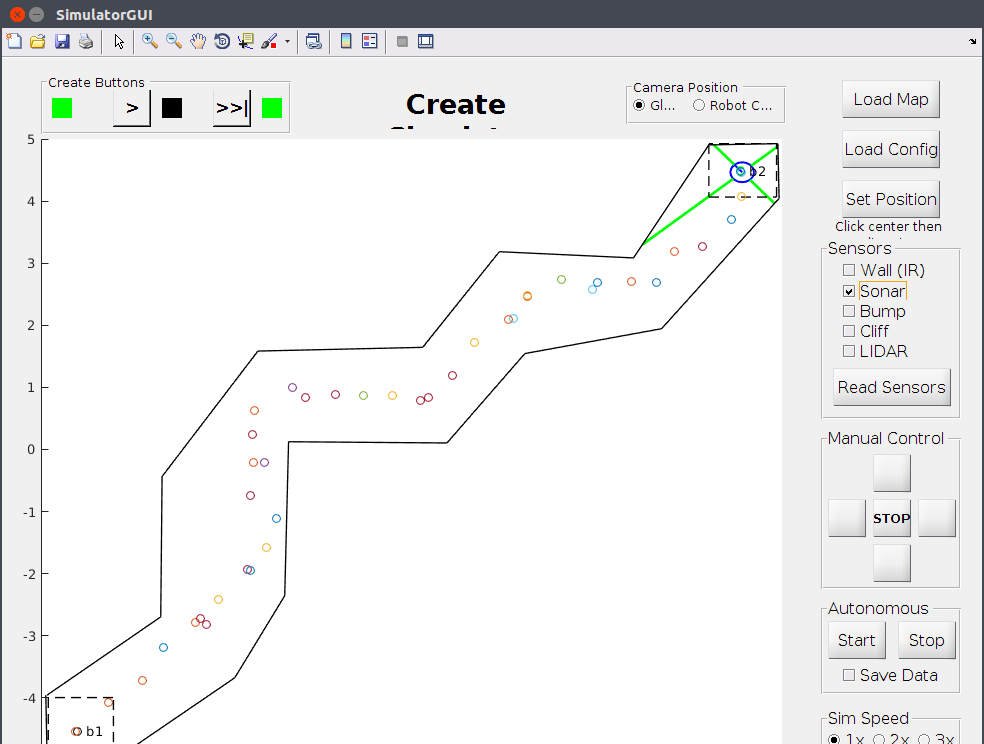
\includegraphics[width=\linewidth]{res1.png}
		\caption{Cap}
		\label{fig:numeros}
	\end{figure}
	
	Projeto 3 IA artigos pesquisados \cite{DUMMY:1, DUMMY:2}\\	
	\bibliographystyle{ieeetr}
	\bibliography{projeto3}
\end{document}